\section{Method}
A controlled trial was designed, whereby the subjects were randomly, but with an equal gender distribution, assigned into a control and treatment group.

\subsection{Subjects}
40 healthy subjects with a normal BMI and an equal gender distribution were recruited (age: 2X$\pm$XX years). 
Excluded were subjects with ongoing meditation practice, acute or chronic pain, neurological, musculoskeletal or mental illness, pregnancy or medications that might influence the subjects’ response to pain.

\subsection{Experimental Procedure}
Testing points, which can be seen on \ref{fig:trapezius}, were marked at the left and right upper trapezius (UT) to ensure reliable and rapid location during the experimental procedure. The baseline values of Pressure Pain Threshold and Pressure Pain Tolerance were measured with an algometer (Wagner Force Ten™ Digital force Gage) four times.  The mean of four measurements, two on each UT, was computed. 

\begin{figure}[H]
\centering
%\caption{} \vspace{-.25cm}
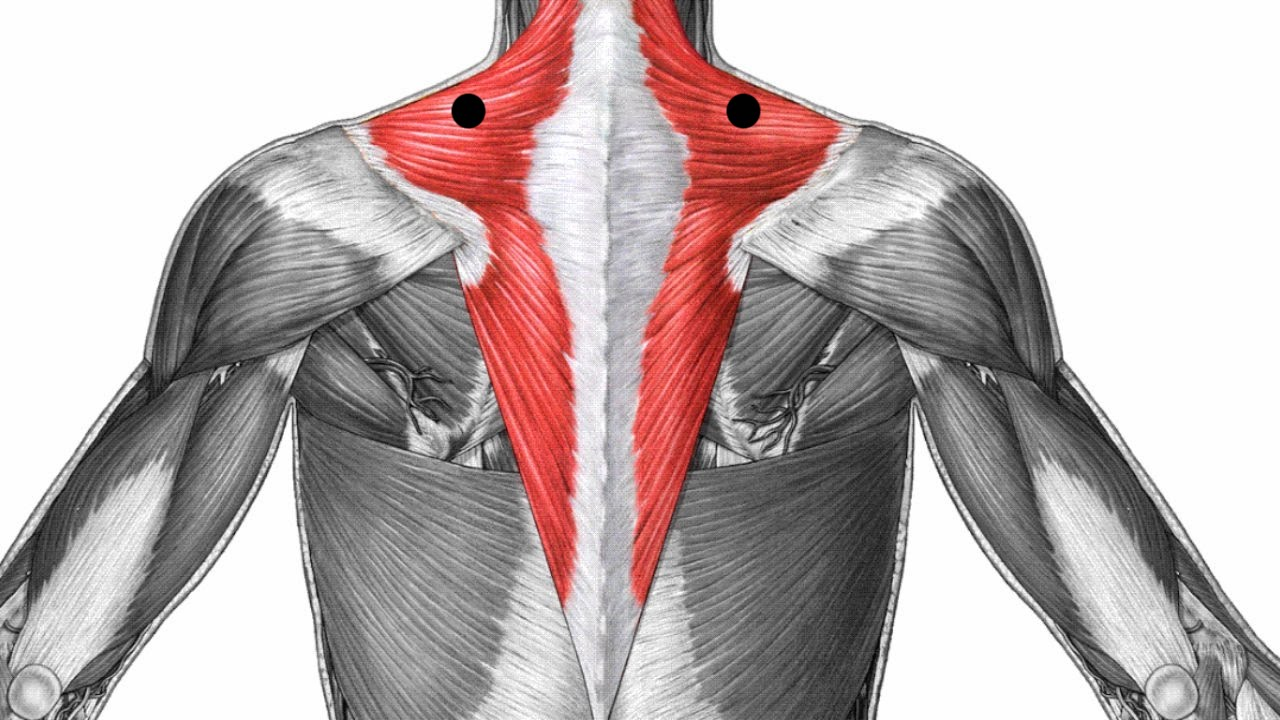
\includegraphics[width=.7\columnwidth]{../figures/trapezius}
\caption{Testing points on the upper trapezius.}
\label{fig:trapezius}
\end{figure} \vspace{-.5cm}

The treatment group practiced 20 minutes mindfulness meditation on 5 consecutive days. After the last meditation session the second measurement was conducted likewise the baseline measurement.
The subjects of the control group continued their normal routine. The same time interval between baseline and second measurement was used for the subjects of the control group.

\subsection{Meditation Technique}
Short-term mindfulness meditation with 20 minutes of meditation on 5 consecutive days.
To ensure same meditation conditions, a guided meditation in form of an audio file was used. A short introduction to mindfulness meditation was provided before the first meditation session.
Here / In this section is missing a little bit! Maybe about FA

\subsection{Data Analysis}
To test the effect of mindfulness meditation on chronic neck pain, a paired t-test / Mann-Whitney / Wilcoxon rank test was applied to the baseline and second measurement of both groups, the treatment and the control group.
